\section{Experiment P1F-G: scalable and diversity-guarded AACOPF}
\subsection{Purpose and adaptation}
P1F-G is the final AACOPF experiment in Phase~1. It addresses two structural limitations identified by P1F-D--P1F-F: the quadratic all-pairs cost of the literal transition and the tendency of unrestricted particle copying to destroy rare useful support or amplify a temporarily wrong mode.

The P1F-G transition is an explicit thesis adaptation, not a literal reproduction of Han et al. Each source particle scores only a global pool of the \(K\) highest-weight particles. Strictly higher-weight members of that pool remain admissible destinations and use the frozen P1F-C score
\begin{equation}
    s_{ij}
    =
    \left(w_j-w_i+\epsilon_w\right)^{\alpha}
    \left(\frac{1}{d_{ij}+\epsilon_d}\right)^{\beta},
    \qquad
    (\alpha,\beta,c_\lambda)=(0.5,0,2).
\end{equation}
Because \(\beta=0\), the frozen transition is purely weight driven. Candidate scoring is therefore reduced from dense \(O(N_p^2)\) scoring to \(O(N_pK)\), plus sorting of the particle weights.

The literal threshold normalization is retained,
\begin{equation}
    \lambda_i=\frac{c_\lambda}{K_i},
\end{equation}
where \(K_i\) is the total number of strictly higher-weight particles in the complete cloud rather than the truncated candidate-pool size. This distinction is important: an early implementation that used the bounded candidate count inflated \(\lambda_i\) and almost suppressed particle movement. The final campaign preserves the literal threshold scale while truncating only destination scoring.

Two explicit diversity guards are added after the score-threshold test:
\begin{enumerate}
    \item a \emph{move cap}, limiting the fraction of sources replaced in one update;
    \item a \emph{destination-capacity limit}, bounding the number of incoming copies received by any one destination.
\end{enumerate}
All accepted moves remain synchronous and copy from the immutable pre-transition cloud.

\subsection{Development selection}
The development sweep uses the controlled 400-particle two-mode benchmark and new seeds 400--407. The grid contains 27 combinations,
\[
K\in\{8,16,32\},\qquad
f_{\mathrm{move}}\in\{0.10,0.25,0.50\},\qquad
f_{\mathrm{dest}}\in\{0.01,0.025,0.05\}.
\]
A candidate must first achieve at least \(90\%\) correct-mode lock and no more than \(5\%\) wrong-mode lock. The predefined safety-first rule then minimizes catastrophic ancestry collapse, dominant cloning, candidate count, and guard sizes.

The selected configuration is
\begin{equation}
    \boxed{
    K=8,\qquad
    f_{\mathrm{move}}=0.10,\qquad
    f_{\mathrm{dest}}=0.025.
    }
\end{equation}
Across the 16 development runs it achieves 16/16 correct locks, 0/16 wrong locks, no catastrophic ancestry collapse, and no dominant-clone event.

\subsection{Held-out controlled ablation}
Table~\ref{tab:p1fg_controlled} separates candidate truncation from the two diversity guards on held-out seeds 500--519.

\begin{table}[htbp]
    \centering
    \caption{P1F-G held-out controlled ablation over 40 runs.}
    \label{tab:p1fg_controlled}
    \begin{tabular}{lrrrrr}
        \toprule
        Method & Correct lock & Wrong lock & Collapse & Dominant clone & Runtime [s]\\
        \midrule
        Conventional PF       & 1.000 & 0.000 & 0.000 & 0.000 & 0.0235\\
        Literal AACOPF        & 0.950 & 0.000 & 0.100 & 0.750 & 0.9872\\
        Candidate only        & 0.450 & 0.525 & 1.000 & 1.000 & 0.0404\\
        Move guard only       & 1.000 & 0.000 & 0.000 & 0.000 & 0.0513\\
        Destination guard only& 1.000 & 0.000 & 0.000 & 0.000 & 0.0634\\
        Fully guarded         & 1.000 & 0.000 & 0.000 & 0.000 & 0.0561\\
        \bottomrule
    \end{tabular}
\end{table}

Candidate truncation alone is not a safe scalability mechanism. It produces catastrophic ancestry collapse and a dominant clone in every held-out run and finishes in wrong-mode lock in \(52.5\%\) of runs. By contrast, either diversity guard restores 40/40 correct locks in this controlled benchmark. The fully guarded method has minimum unique-parent fraction \(0.975\); the destination-capacity guard is therefore the dominant genealogy-preservation mechanism in this experiment.

\subsection{Held-out random-annulus global validation}
The selected guarded transition is next tested on new seeds 600--619 with the full random first-range annulus plus random-yaw initialization, informative moving geometry, exact paper-level motion increments, and matched PF/AACOPF initial clouds and UWB realizations. Conventional PF is run with zero \(\Delta L\) and \(\Delta\phi\) process noise, matching the P1F-D reference.

\begin{table}[htbp]
    \centering
    \caption{P1F-G held-out global random-annulus validation.}
    \label{tab:p1fg_global}
    \begin{tabular}{rrlrrr}
        \toprule
        \(N_p\) & Method & Success & Late pos. RMSE [m] & Late yaw RMSE [deg] & Runtime [s]\\
        \midrule
        1200  & PF              & 1/20 & 14.812 & 46.687 & 0.255\\
        1200  & Guarded AACOPF  & 0/20 & 10.699 & 32.638 & 0.570\\
        1200  & Candidate only  & 0/20 & 36.096 & 111.593 & 0.501\\
        5000  & PF              & 2/20 & 10.275 & 28.331 & 0.802\\
        5000  & Guarded AACOPF  & 2/20 & 8.000  & 22.672 & 1.797\\
        10000 & PF              & 3/20 & 10.017 & 29.514 & 1.525\\
        10000 & Guarded AACOPF  & 1/20 & 7.043  & 19.501 & 3.439\\
        \bottomrule
    \end{tabular}
\end{table}

The diagnostic correct-region support grows from 2.75 particles on average at \(N_p=1200\), to 9.85 at \(N_p=5000\), and 19.0 at \(N_p=10000\). Nevertheless, the guarded transition does not improve strict global-pose acquisition: it loses the single PF success at \(N_p=1200\), ties PF at \(N_p=5000\), and achieves 1/20 versus 3/20 PF successes at \(N_p=10000\).

The guarded method does reduce mean late position and yaw error at every tested population. This is retained as an error-shaping effect, not a convergence claim. The candidate-only result at \(N_p=1200\) is an important negative ablation: computational truncation without explicit diversity control is substantially worse than either PF or the guarded method.

\subsection{Computational scaling}
The bounded transition and literal all-pairs transition are timed separately at the single-transition level. The bounded empirical log--log runtime slope over \(N_p\in\{400,1200,5000,10000,40000\}\) is \(0.926\), whereas the literal reference over \(N_p\in\{100,200,400,800,1200\}\) has slope \(1.947\).

At \(N_p=40000\), the bounded transition has median runtime approximately \(\SI{0.0281}{s}\) and evaluates 319964 candidate scores. A dense all-pairs representation would contain \(1.6\times10^9\) pairs, so the bounded implementation scores only about \(0.020\%\) of the hypothetical dense pair count. This establishes the scalability claim independently of the filtering-accuracy result.

\subsection{P1F-G interpretation}
P1F-G supports two claims and rejects a third:
\begin{itemize}
    \item \textbf{Scalability is supported:} bounded candidate scoring removes the dense all-pairs bottleneck.
    \item \textbf{Diversity safety is supported:} the explicit guards prevent the catastrophic genealogy collapse seen in literal and candidate-only AACOPF on the held-out controlled benchmark.
    \item \textbf{Improved strict global acquisition is not supported:} the guarded transition does not outperform conventional PF in held-out random-annulus full-pose convergence.
\end{itemize}

The appropriate Phase-1 interpretation is therefore that guarded weight-directed redistribution can be made computationally practical and genealogically safe, and can reduce late estimation error when useful hypotheses survive. It does not remove the fundamental finite-support and global-mode-selection difficulty of unknown-pose localization.

The final corrected campaign is GitHub Actions run \texttt{35068506066}, artifact \texttt{p1f-g-results}, artifact ID \texttt{10435397349}. Compact final evidence is version controlled in \texttt{results/phase1/p1f\_g/}; full per-run evidence remains in the workflow artifact.


\subsection{P1F-G result visualization}
Figure~\ref{fig:p1fg_result} combines the three claims that must remain separate. Candidate truncation alone is unsafe, the diversity guards restore controlled mode selection, bounded/guarded AACOPF lowers late global error without improving strict acquisition, and the bounded transition materially changes computational scaling.
\begin{figure}[htbp]
    \centering
    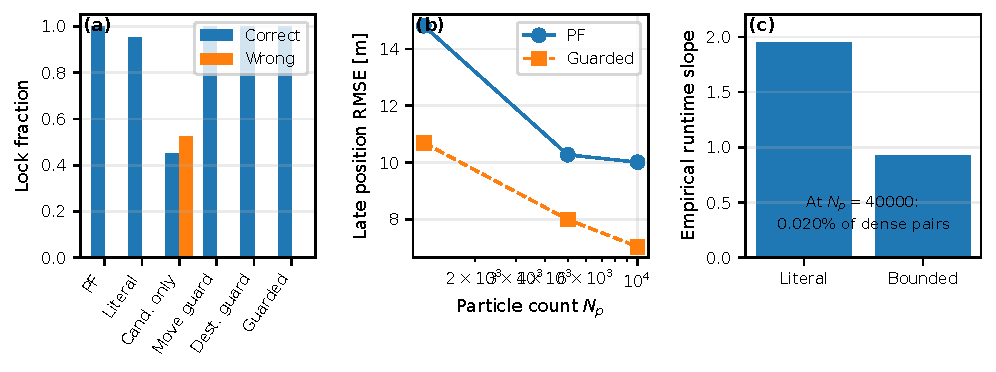
\includegraphics[width=0.99\textwidth]{figures/phase1/p1fg_scalable_guarded.pdf}
    \caption{P1F-G scalable guarded adaptation. (a) Held-out controlled correct/wrong lock fractions across the PF/AACOPF ablation. (b) Mean late position RMSE in the global random-annulus validation. (c) Empirical runtime-scaling slopes for literal and bounded transitions.}
    \label{fig:p1fg_result}
\end{figure}
